
\subsection*{Bizum}
\addcontentsline{toc}{subsection}{Bizum}



Bizum és un proveïdor de serveis de pagament d'Espanya fundat l'any 2016, fruit de la col·laboració de 34 entitats bancàries del país, per crear un sistema de pagaments instantanis entre particulars i de compres a comerços. 

En la següent taula es pot veure que Bizum s'ha expandit ràpidament tenint en compte que la població d'Espanya és de 48 milions d'habitants: 
\begin{table}[h]
    \centering
    \begin{tabular}{|c|c|c|}
        \hline
        \textbf \textbf{Any} & \textbf{Usuaris} \\
        \hline
        2019 & 6 milions \\
        \hline
        2020 & 10 milions \\
        \hline
        2021 & 15 milions \\
        \hline
    \end{tabular}
    \caption{Usuaris de Bizum}
\end{table}

Bizum només està disponible a Espanya. Es pot fer Bizum a un altre país, però cal tenir un compte bancari en una entitat espanyola. Aquest és l'únic requisit per continuar fent servir Bizum fora d'Espanya. I de la mateixa manera només podràs fer pagaments amb Bizum a números vinculats a un compte d'un banc espanyol.







\subsection*{Cartera digital}
\addcontentsline{toc}{subsection}{Cartera digital}

Cartera digital és un servei de pagament mòbil i cartera digital. Un cop vinculada la targeta, ja es pot començar a utilitzar l'aplicació, tan sols amb el telèfon mòbil i incorporant les mesures de seguretat de la pròpia. Però la firma vol anar un pas més enllà, i ja està introduint pagaments amb reconeixement facial en alguns comerços, de manera que ja ni tan sols calgui utilitzar el telèfon intel·ligent en el procés de pagament. Segons Merchant Savvy, el 2022 l'ús global de pagaments mòbils superarà el de les targetes de crèdit i l'efectiu.
Els més utilitzats són:

\begin{itemize}
    \item paypal neix en 1998: unit al fet que facilita la compra amb targetes estrangeres fins i tot en llocs web amb limitacions geogràfiques, ha contribuït al continu creixement del nombre de comptes actius de Paypal que al tancament del 2022 se situaven per sobre dels 435 milions.
    \begin{figure}[h]
        \centering
        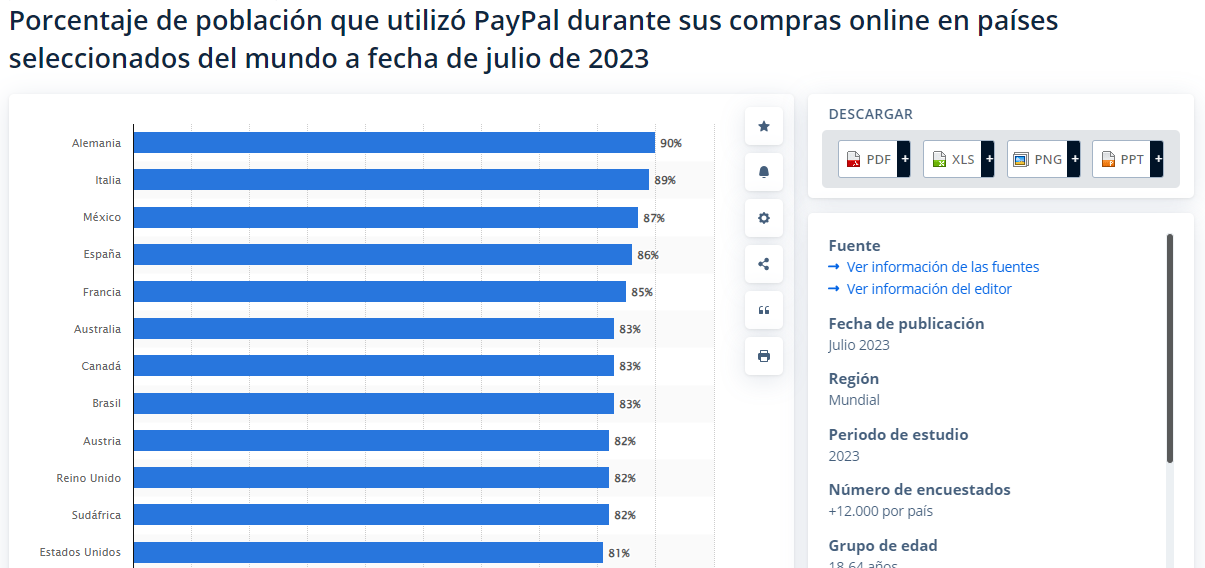
\includegraphics[width=8cm]{usuarispaypal.png}
        \caption{Primera tarjeta bancaria}
    \end{figure}  
    \\
    \\
    \\
    \\
    \\
    \\
    \item Google Pay neix en 2011: té actualment 100 milions d'usuaris i s'estima que el 12\% de la població mundial fa servir regularment aplicacions d'e-wallets. 
    \begin{figure}[h]
        \centering
        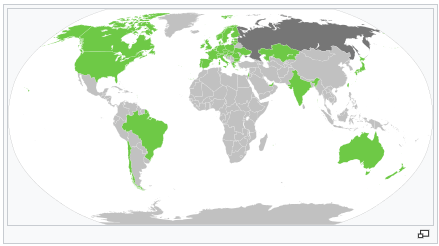
\includegraphics[width=8cm]{disponiblitatgooglepay.png}
        \caption{Primera tarjeta bancaria}
    \end{figure}  
    \item Apple Pay neix en 2014: té 507 milions d'usuaris a tot el món i comptant. S'estima que el 12\% de la població mundial utilitza regularment aplicacions de cartera digital.
    \begin{figure}[h]
        \centering
        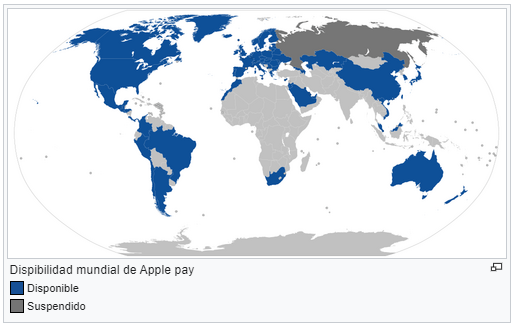
\includegraphics[width=8cm]{didponiblitatapplepay.png}
        \caption{Primera tarjeta bancaria}
    \end{figure}  
\end{itemize}












